\section{Case Study and Statistical Analysis} \label{sec:app}

\subsection{Case Study - JPEG}
To demonstrate the efficacy of the proposed scheme we use as case study the JPEG, which is a widely used    
lossy compression technique of digital images that became a popular application example among error resilient techniques.  
JPEG consists of several stages including color space transformation and down sampling. In this work, we focus on the subsystem shown in Figure \ref{fig:qos_jpeg} which consists of four major procedures. In particular an input image of size $512 \times 512$
is decomposed into 4,096 matrices of the size $8 \times 8$. Then each matrix is being processed individually by the 2D Discrete Cosine Transformation (2-D DCT) \cite{gonzalez2009digital} that essentially  transforms the image into the frequency domain producing the DCT coefficients as output which are then finally being quantized. For the reconstruction of the image De-quantization and 2D Inverse Discrete Cosine Transformation (2-D IDCT) are applied. In general, the quality of the output image compared to the original one is evaluated using the peak signal to noise ration (PSNR) \cite{huynh2008scope} and a typical PSNR value for a lossy image is 30 dB. 

\begin{figure}
\centering
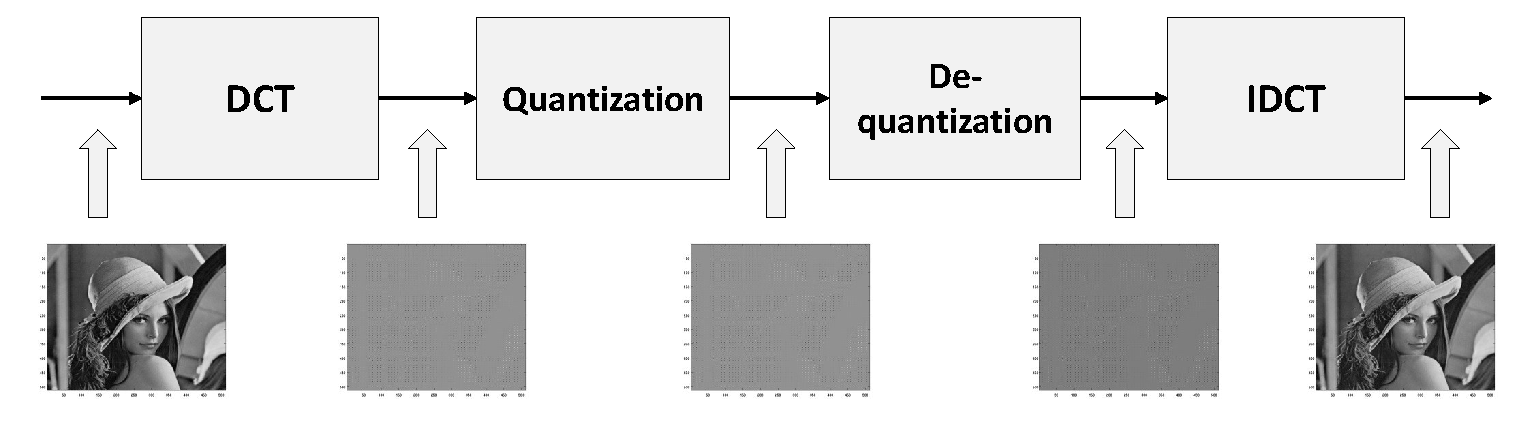
\includegraphics[width=80mm]{./eps/qos_jpeg}
\caption{Subsystem in JPEG application}
\vspace{-4mm}
\label{fig:qos_jpeg}
\end{figure}

\subsection{Statistical Analysis of JPEG}
Following the steps of the proposed approach we statistically analyzed the different stages of JPEG by performing several simulations with different images. Simulations show that the output matrices of DCT and quantization share a similar pattern; the elements at the top-left corner of both DCT and quantization output matrix are larger in magnitude compared to the rest which in most cases are close to zero. Figure \ref{fig:qos_matrix} shows the expected value of each element in the DCT and quantization 
output matrix after averaging their values across 4,096 individual matrices for over 10 images. Such values are used as the reference expected values for replacing the erroneous data in case of a detected memory error in our approach. Note that these values are stored in a LUT that was described in Section III. 

\begin{figure}
\centering
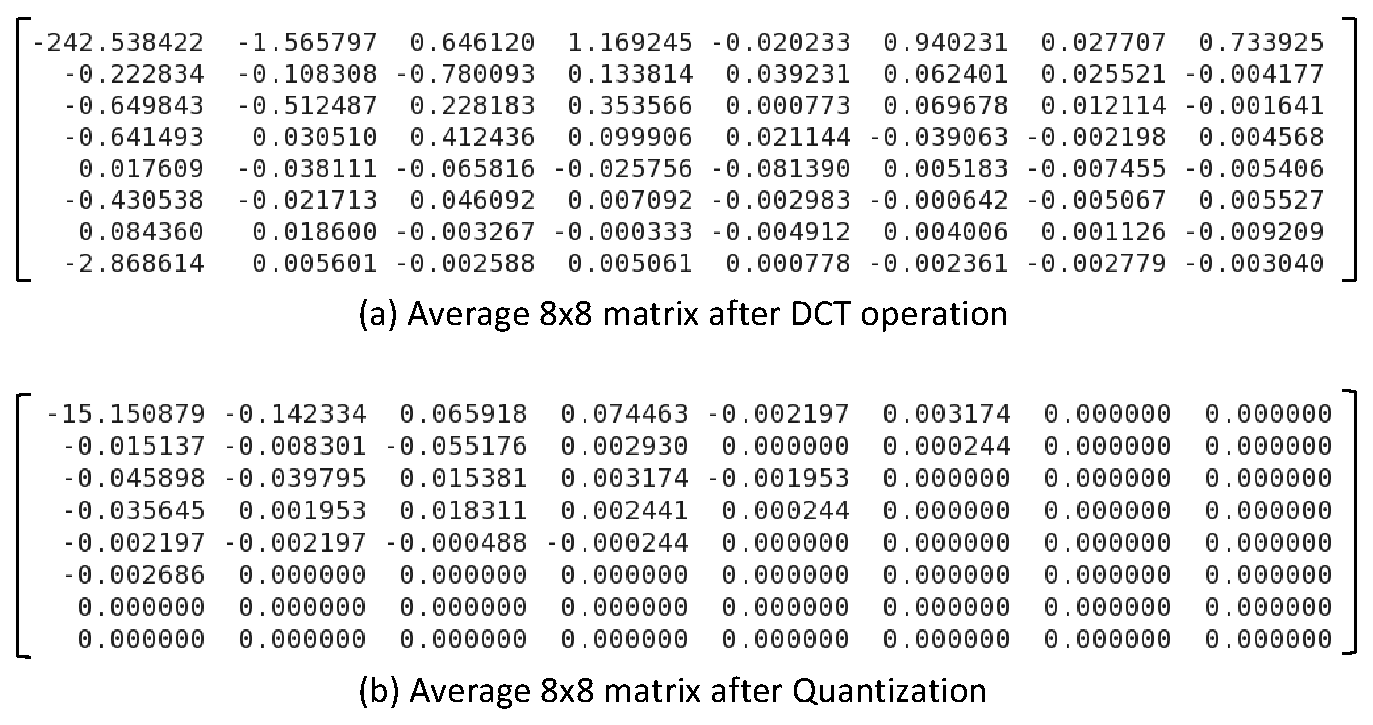
\includegraphics[width=80mm]{./eps/qos_matrix}
\caption{Reference matrix for DCT and Quantization Coefficients}
\vspace{-4mm}
\label{fig:qos_matrix}
\end{figure}


\section{Results} \label{sec:exp}

\subsection{Experimental Setup}
We have modified the RISC processor as discussed in Section II and enabled the injection of bit flips in the memory
locations storing the images and intermediate results of the JPEG. Note that no errors are injected on instruction cache and other registers which are assumed to be adequately protected.     

For detecting errors as we said we encoded each of the 32-bit data of the application with a single parity bit which is sufficient for detecting a single fault. Following the proposed method the new instructions were used as inline assembly to describe JPEG as shown in Figure \ref{fig:qos_program}.  In this example an array containing the reference expected values for the DCT coefficients is defined. 
Within the DCT function, before performing a store to the memory, parity encoding is enabled, which is turned off after a write-store operation. Within the quantization function, the load check is performed whenever a value is read out from the array where the DCT coefficients are stored for replacing it with the relevant expected value in case of an error.

\begin{figure}
\centering
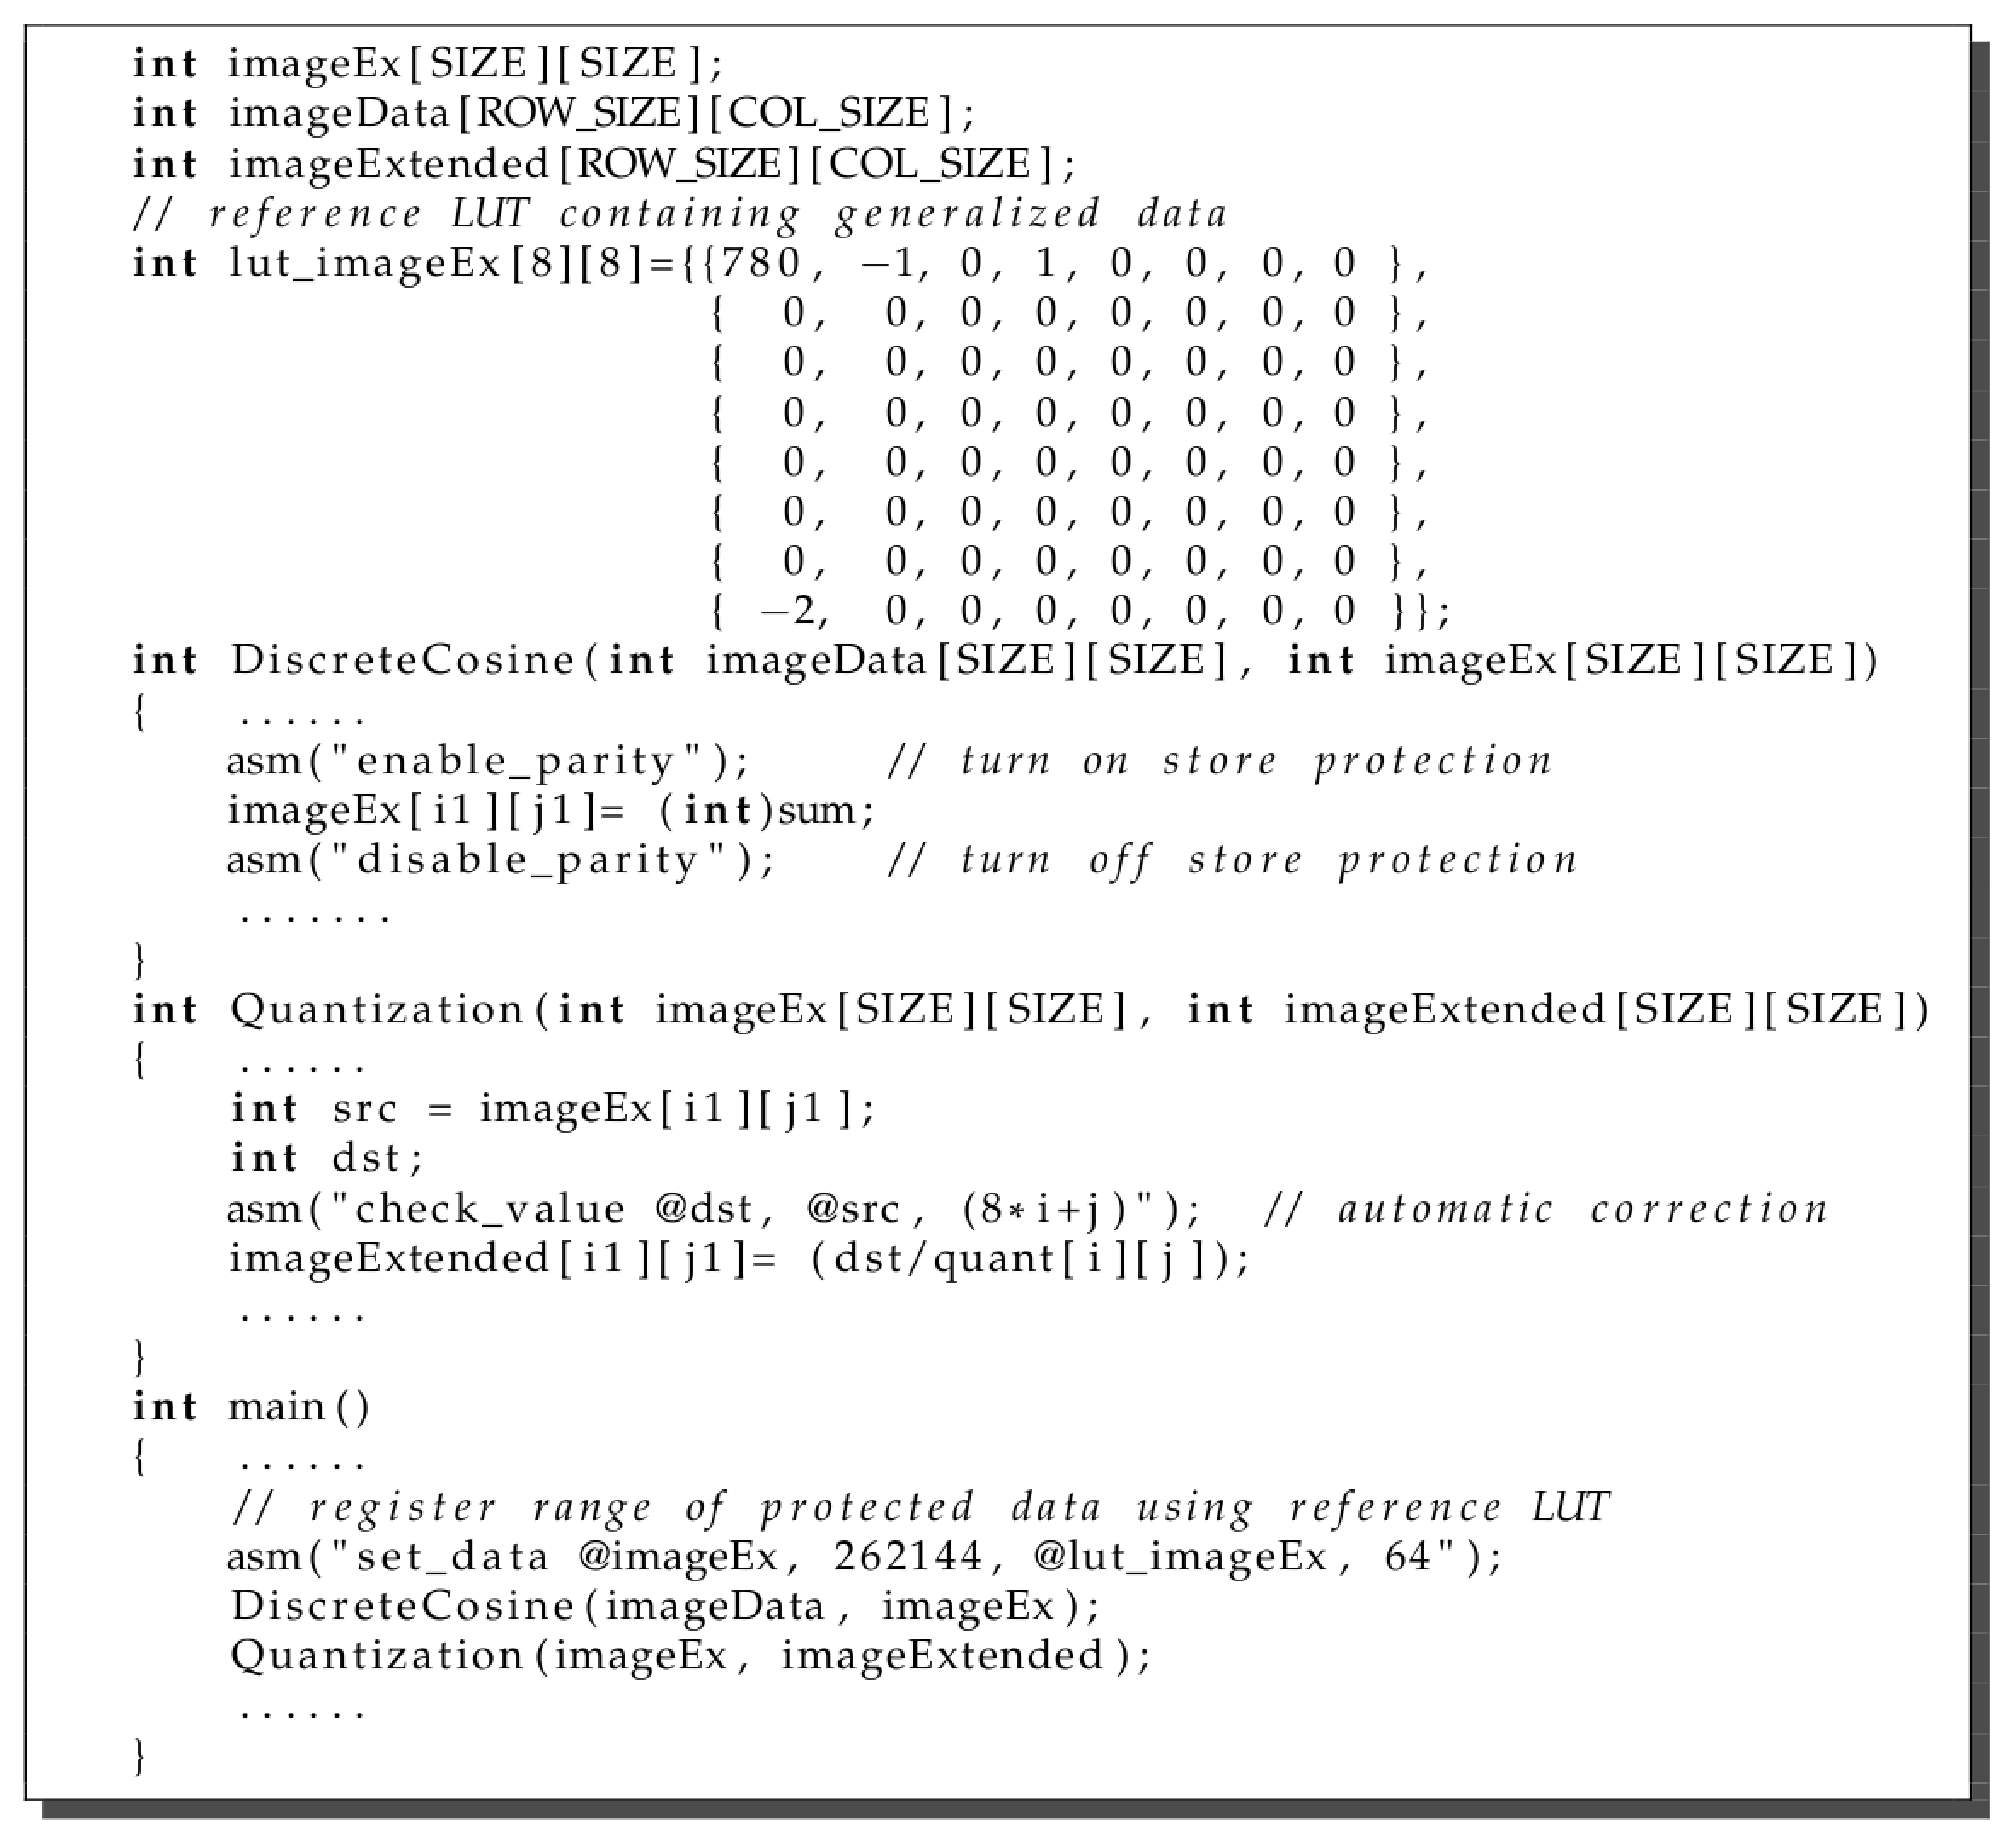
\includegraphics[width=80mm]{./eps/qos_program}
\caption{Programming example with custom instructions for DCT}
\vspace{-4mm}
\label{fig:qos_program}
\end{figure}

The above code was compiled and executed on the modified processor and the performance, power and quality were measured under different error rates as discussed next. Note that for comparison we replicated a similar infrastructure by using a conventional SECDED Hamming code scheme $H[38, 32]$ for the protection of the specific memories (protected by our scheme), which requires 6 parity bits for encoding each 32 bit memory word.  

\subsection{Evaluation of Quality}

Figure \ref{fig:qos_lena} shows the output images and corresponding PSNR values with different numbers of injected bitflips according to typical error rates in 65nm process technology. The results show that in case of 800 and 1000 bitfilps, the output image is degraded by 7.6\% and 41.2\% compared to the error free case.
 
The reason for such a large degradation in case of 1000 bitflips is that two bitflips in the same data word are allowed
which cannot be detected by the single bit parity. Careful examination of our simulations indicated that some of such double bitflips affected words that relate to the first 20 DCT coefficients of the $8 \times 8$ matrix (remember there are 4092 such matrices in each image). As other works have also shown such coefficients control almost 85\% of the overall image quality and thus if the get affected by errors and these are not tackled by any means as in this case then they lead to significant quality degradation. 

\begin{figure}
\centering
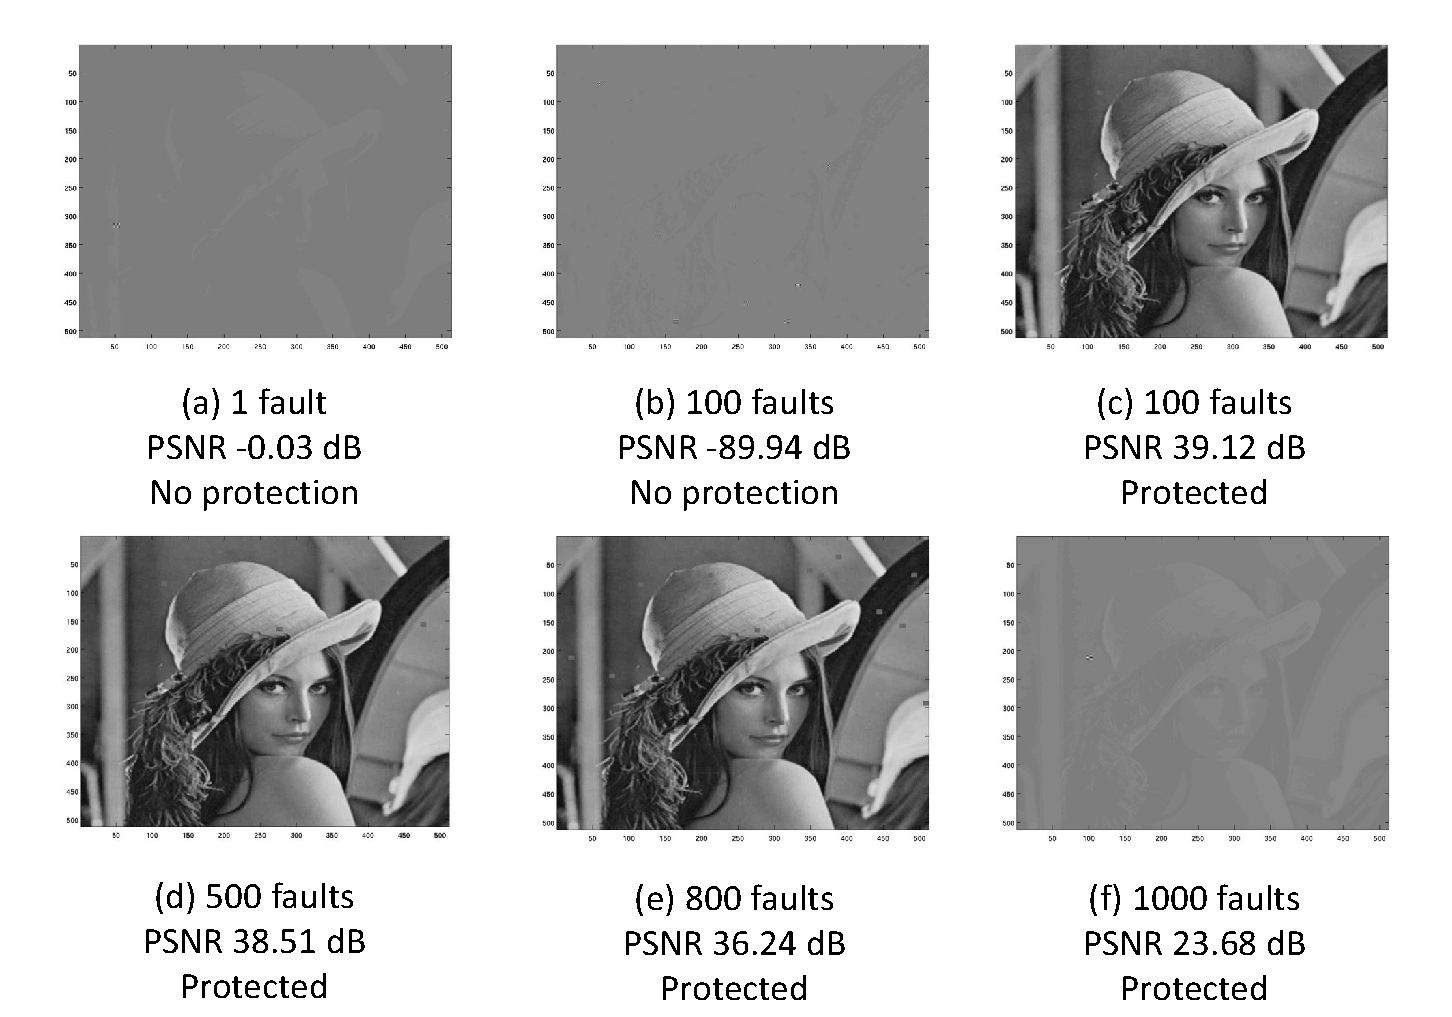
\includegraphics[width=80mm]{./eps/qos_lena}
\caption{Output images under different schemes of error injection}
\vspace{-4mm}
\label{fig:qos_lena}
\end{figure}

As we mentioned we compared the quality achieved by our approach with a SECDED ECC.   
Figure \ref{fig:qos_snr} shows the obtained results in case of protecting the output DCT and quantization coefficients wth the two schemes under different number of single bitflips.  We observed that as the number of the injected single bitflips increases, the output quality (interms of PSNR) achieved by using the proposed approach is slightly less than that achieved by using the ECC scheme. This can be attributed to the fact that in some cases the correct value of the erroneous data that is being substituted by the expected value may indeed lie in the tale of the distribution and thus may be far from the used reference expected value. In these cases the replacement will not be as accurate and thus the quality achieved by our approach may not be as perfect. In any case as we discussed our approach tries to confine the impact of memory errors by essentially approximating erroneous data with their expectation and sometimes such an approximation may not be as good. However, note that the proposed approach still achieves to provide output images with PSNR above 36 dB even under 800 bitflips, closely approximating the error free image.

We observed that above 800 bitflips (when double bitflips are allowed in each word) both methods fail to produce a good enough   image, since neither scheme is able to detect and mitigate from multiple bitflips in single data word. In particular, on one side the SECDED ECC intrinsically cannot correct more than one error in a word and on the other side the single parity bit used to in the proposed scheme cannot detect two bitflips in a word and thus it does not engage the replacement of the erroneous data.

Our results reveal also a different aspect in the JPEG application. In particular, we observed that in case of more than 800 bitflips when double bitflips are taking place in each word then any untreated error in quantization coefficients are far more severe (causing large quality degradation) compared to untreated errors in DCT coefficients. 
This can be attributed to the sparse nature of the quantization coefficients (i.e. most of them are zero) and thefact that any untreated error will significantly alter the expected distribution of these data. 

\begin{figure}
\centering
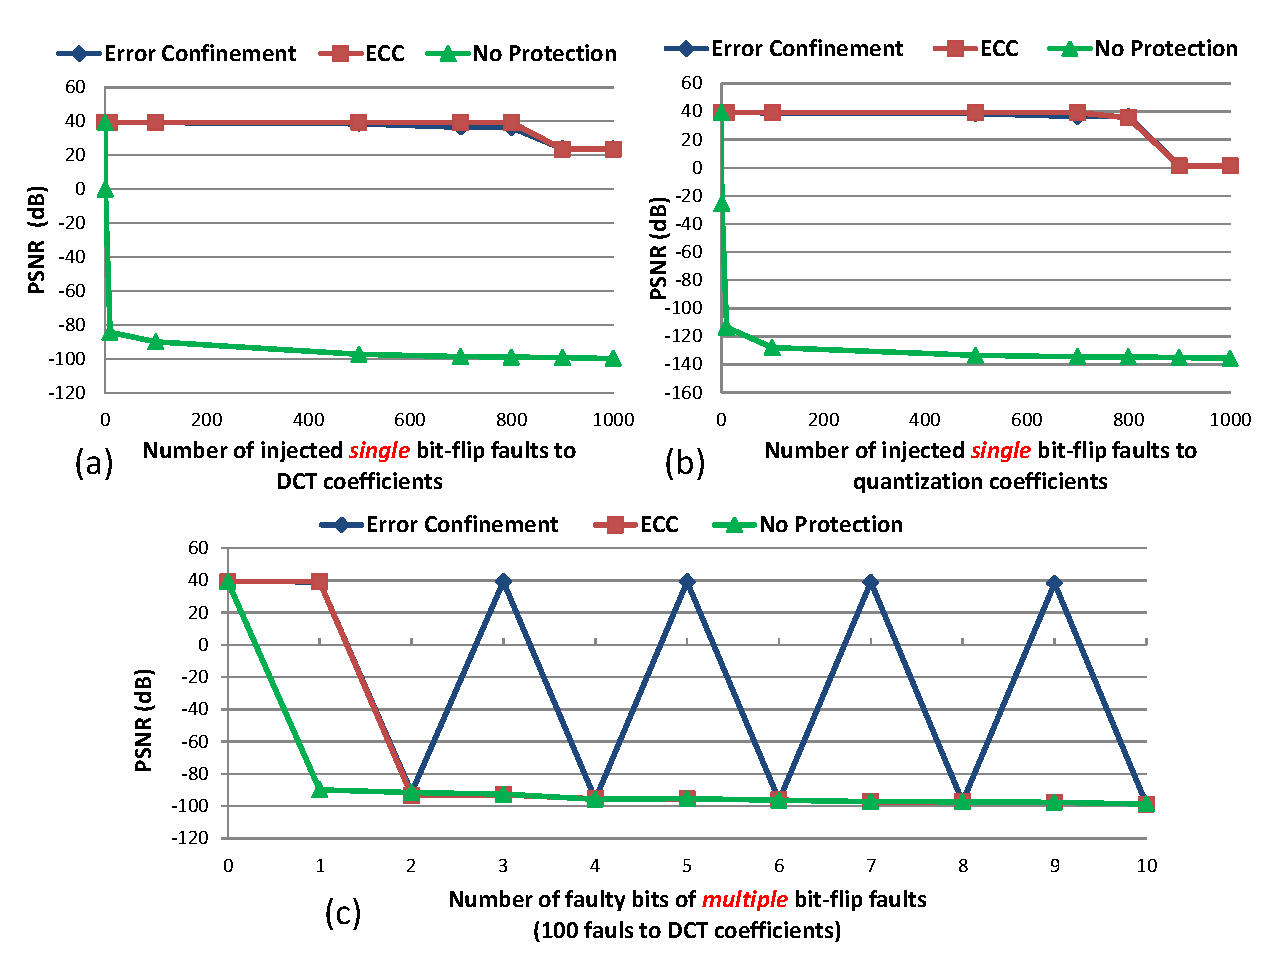
\includegraphics[width=90mm]{./eps/qos_snr}
\caption{PSNR under no protection, proposed scheme and ECC}
\vspace{-4mm}
\label{fig:qos_snr}
\end{figure}

In addition to the above experiments, we have also evaluated the ability of our approach to address multiple bitflips in a single data word by replacing it with the expected reference value. Figure \ref{fig:qos_snr}c) shows the achieved PSNR under different number of bitflips in each word. We can observe that the proposed scheme helps to obtain a PSNR of more than 38dB (for the particular image) in case of odd number of faulty bitcells (when the parity bit can detect the error) while the PSNR degrades a lot in case of even number of faulty bit cells (which cannot be detected by a single parity bit). On the contrary, note that the SECDED ECC even with the use of 6 parity bits fail to address any number of multi bitlfips requiring more complex ECC schemes with much more parity bits. All in all, the proposed approach even with the use of single parity bit is able to address adequately the cases of odd multi flipbits in a single word. The addition of another parity could be employed to improve the capability of error detection which is left for future experimentation. The essential conclusion is that the replacement      
of erroneous data with an expected value suffices to confine the impact of single or even multi memory bitflips.  

\subsection{Performance and Power Results} \label{sec::soft_overhead}
The proposed enhanced processor is synthesized in 65nm Faraday technology and the power, performance and area results
compared to  the original processor are shown in Table \ref{tab:qos_overhead}. Note that the reference processor in this case does not employ any protection scheme and our results in this paragraph try to reveal the overheads involved in enabling 
preferential protection of specific parts of a memory with special instructions as well as the cost of the proposed data replacement scheme.  We can observe that the performance is decreased by only 4.2\% but the instruction extensions for realization of the proposed scheme by a generic programming environment have resulted in large power and area overheads. The extra logic and registers for specifying the protected memory addresses (which is a unique and desirable feature in todays error resilient systems enabled by the proposed extensions), the added LUT and the 1-bit parity encoding are responsible for such overheads. However, note that implementing the same instruction extensions by using 6parity bits as needed by a H(38,32) ECC will result in much larger overheads. 

\begin{table}[hbt]
\begin{center}
\caption{Results for the proposed architecture extensions compared to the reference unprotected processor }
     \label{tab:qos_overhead}
\begin{tabular}{|c|c|c|c|c|c|}\hline 
                  & \multicolumn{2}{c|}{\textbf{Area}} & \multicolumn{2}{c|}{\textbf{Power}} & \textbf{Critical} \\ 
                  & \multicolumn{2}{c|}{\textbf{(NAND equiv.)}} & \multicolumn{2}{c|}{\textbf{($\mu$Watt)}} & \textbf{path} \\ %%\cline{2-5}
                  & Comb. & Seq. & Dynamic & Leakage & (ns) \\\hline
Original          & 11789         & 6187       & 206     & 65      & 6.12 \\\hline
Proposed extensions     & 26519         & 10663      & 349     & 124     & 6.38 \\\hline
Increase (\%)     & 124.9         & 72.3       & 69.4    & 90.8    & 4.2  \\\hline
\end{tabular}
\end{center}
\end{table}

To compare with the SECDED ECC we show the total time required for executing the JPEG application on a processor instance that involves our scheme and on another that implements the ECC. Figure \ref{fig:qos_time_size} depicts the overall execution time of the JPEG application after processing images of different sizes from $8 \times 8$ till $1,024 \times 1,024$ and correcting randomly injected errors (in same locations) with ECC and the proposed scheme.

For small images both methods take similar time since the modules other than the ones shown in Figure \ref{fig:qos_jpeg} dominate the execution time. For images larger than $64 \times 64$ ECC takes significantly longer time compared to proposed scheme. In particular, for an image of size $1,024 \times 1,024$, ECC takes \textbf{3.5}$\times$ more time than the proposed scheme. Note that such overhead will further increase for larger images and more injected errors. 

\begin{figure}
\centering
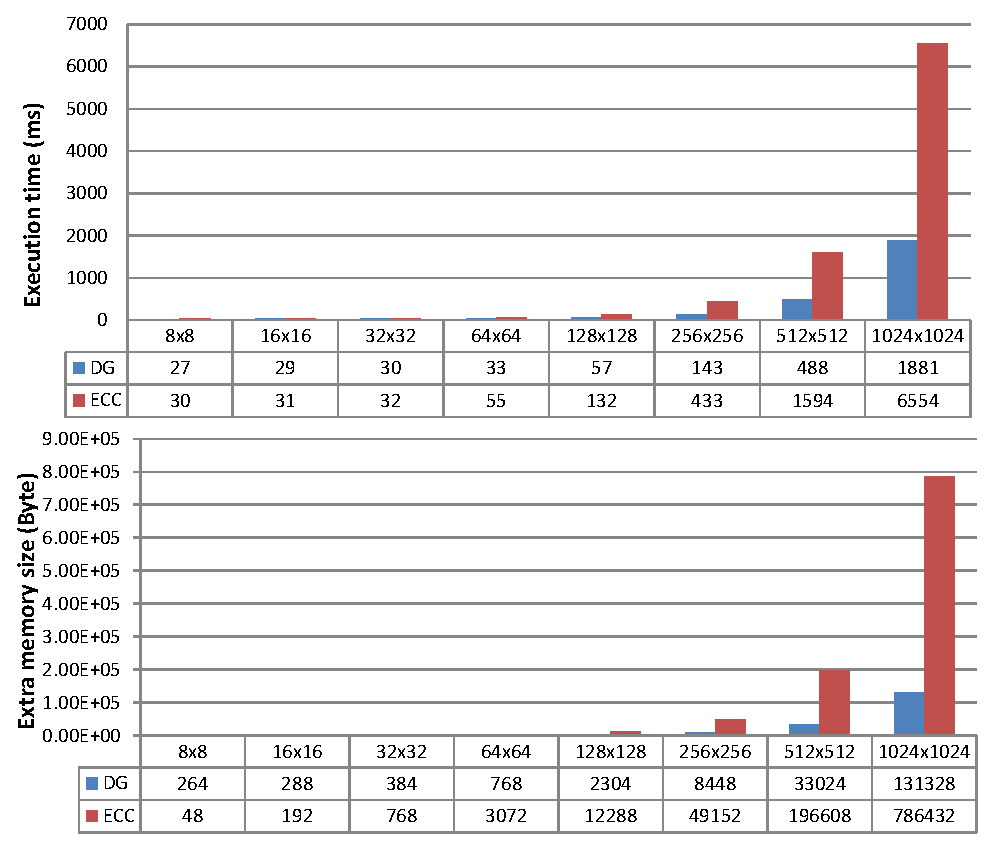
\includegraphics[width=70mm]{./eps/qos_time_size}
\caption{Execution time and data memory usage under Error Confinement and ECC}
\vspace{-4mm}
\label{fig:qos_time_size}
\end{figure}

Although the architecture extension achieves large power overhead, the energy consumption ratio between proposed approach and ECC reduces as image size grows, which is illustrated in Figure \ref{fig:qos_energy}. This is because ECC takes longer time to finish. Starting from image size of $128 \times 128$ the proposed approach consumes less energy than ECC, while the energy benefit increases even further for larger images.

\begin{figure}[hbt]
\centering
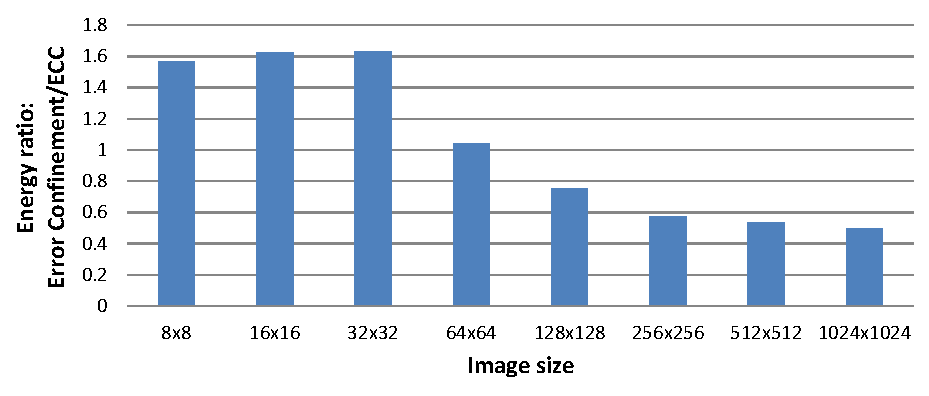
\includegraphics[width=70mm]{./eps/qos_energy}
\caption{Energy ratio between proposed approach and ECC vs image size}
\vspace{-4mm}
\label{fig:qos_energy}
\end{figure}

Another interesting comparison to discuss is the difference in terms of memory usage. As we can also see in Figure \ref{fig:qos_time_size}
the proposed approach uses far less memory compared to SECDED ECC scheme which incurs 18.75\% memory overhead in each protected data word. In particular, for an image of size $1,024 \times 1,024$, ECC requires \textbf{5.99}$\times$ more memory than the proposed error confinement approach.